\chapter{Production d'une source cohérente d'ondes de matière}
\label{ch:BEC_manip}
%\begin{tikzpicture}[remember picture, overlay]
%\node[anchor=north east,inner sep=0pt] at (current page.north east) {
\includegraphics[scale=1]{Fig/Chapter1/g825.png}};
%\end{tikzpicture}


interaction lumière-atome, BEC, principales étapes de refroidissement. 

Partie précédente = introduction à la physique de cette thèse: propagation d'onde en milieu désordonné. À présent, description de notre source d'ondes de matière: un condensat de Bose-Einstein. Le désordre sera présenté chapitre 4. 

Dans ce chapitre, nous nous attacherons à décrire un condensat de Bose-Einstein et ses principales propriétés, les outils dont nous disposons pour manipuler les atomes, et enfin la manière dont ces outils sont implémentés sur notre expérience.

\section{Condensation de Bose-Einstein}
Commençons par décrire ce qu'est un condensat de Bose-Einstein. Le phénomène de condensation a été prédit par Albert Einstein dans les années 1920 en s'appuyant sur les travaux de Satyendranath Bose traitant des statistiques quantiques pour des particules plus tard appelées \emph{bosons}. Il a cependant fallu attendre les années 1960 et le développement des premiers lasers pour voir émerger les premières techniques de manipulation d'atomes. La mise au point de telles technologies a d'ailleurs valu le prix Nobel à ses principaux architectes Claude Cohen-Tannoudji, Steven Chu et William D. Phillips en 1997. Enfin, le premier condensat de Bose-Einstein gazeux de ${}^{87}$Rb a été obtenu par l'équipe de Eric Cornell et Carl Wieman \citep{anderson1995observation}, rapidement suivi par un condensat de ${}^{23}$Na obtenu par Wolfgang Ketterle \citep{davis1995bose}. Ces travaux ont été récompensés par le prix Nobel de 2001.

\subsection{Statistique de Bose-Einstein}
Le phénomène de condensation de Bose-Einstein trouve son origine dans la statistique de Bose-Einstein. Celle-ci se différencie de la statistique classique de Boltzmann dans le formalisme grand-canonique donnée par:
\begin{equation}
N_{\mathbf{n}}=g_{\mathbf{n}} \exp{\left( -(E_{\mathbf{n}}-\mu)/k_{\mathrm{B}}T \right)}
\end{equation}
pour un gaz de $N$ particules à l'équilibre thermique, avec $N_{\mathbf{n}}$ le nombre moyen d'atomes présents dans l'état d'énergie $E_{\mathbf{n}}$ et de dégénérescence $g_{\mathbf{n}}$, $\mu$ le potentiel chimique, $T$ la température et $k_{\mathrm{B}}$ la constante de Boltzmann. L'origine de cette différence provient de l'indiscernabilité des particules: dans le cadre de la physique classique, les particules identiques sont discernables, c'est à dire qu'il est possible "d'étiqueter" les particules et de suivre leurs mouvements individuels.
Dans le cadre de la mécanique quantique, une telle approche n'est pas possible car les particules sont décrites par des fonctions d'onde, étalées dans l'espace. Lors de collisions de particules identiques, le recouvrement de leur fonction d'onde fait qu'il est impossible de déterminer les trajectoires suivies par les particules. L'indiscernabilité des particules dans le cadre de la mécanique quantique est donc essentielle.

\begin{figure}
\centering
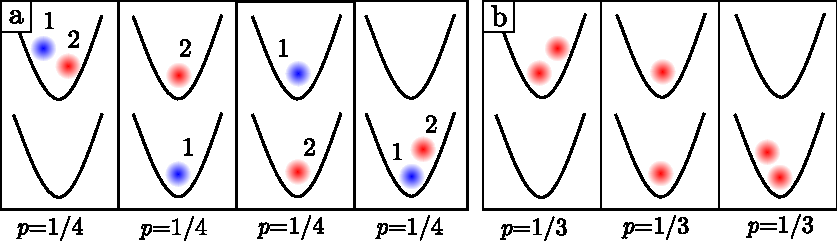
\includegraphics[width=\textwidth]{Fig/BEC_manip/stat_bose.pdf}
\caption{\textbf{a}: Répartition de deux particules discernables numérotées 1 et 2 sur deux niveaux d'énergie. Quatre configurations sont possibles. \textbf{b}: Répartition de deux particules indiscernables sur deux niveaux d'énergie. Dans le cas où ces particules peuvent se trouver dans le même état (bosons), trois configurations sont alors possibles.}
\label{fig:stat_bose}
\end{figure}

Considérons alors le cas simple de la répartition de deux particules sur deux niveaux d'énergie. Dans le cadre de la physique classique, il est possible d'attribuer un numéro à chaque particule, et il on peut placer chaque particule dans n'importe quel niveau d'énergie. Il existe alors quatre configurations que l'on supposera équiprobables, chacune de probabilité $p=1/4$ (voir figure \ref{fig:stat_bose}a). L'approche quantique, dans laquelle il n'est pas possible de discerner les particules, restreint le nombre de possibilités à trois et donc la probabilité de chacune des configurations est alors de $p=1/3$ (voir figure \ref{fig:stat_bose}b). Calculons maintenant la probabilité que deux particules soient dans le même état. En physique classique, cette probabilité est de $p=2/4=1/2$, tandis qu'en mécanique quantique, celle-ci est de $p=2/3$. On s'attend alors à ce que l'indiscernabilité des particules en mécanique quantique modifie la statistique de Boltzmann en favorisant l'agrégation de particules dans le même état \footnote{Ce raisonnement est valable pour des particules bosoniques, qui peuvent se retrouver dans le même état quantique. Pour des particules fermioniques, qui ne peuvent pas se retrouver dans le même état quantique, les statistiques en sont donc profondément changées. En guise d'illustration, la seule configuration possible de la figure \ref{fig:stat_bose}b pour des fermions est la seconde configuration.}.

\paragraph*{Condensation de Bose-Einstein}
Considérons alors le cas d'un gaz de $N$ bosons identiques dans un piège harmonique:
\begin{equation}
V(x,y,z)=\frac{1}{2}m \omega_x^2 x^2 + \frac{1}{2}m \omega_y^2 y^2 + \frac{1}{2}m \omega_z^2 z^2
\label{eq:piege_harmonique}
\end{equation}
où $m$ correspond à la masse des particules, et les $\omega_i$ correspondent aux fréquences de piégeage dans chaque direction de l'espace. Les énergies $E_{\mathbf{n}}$ sont donc celles des états liés
\begin{equation}
E_{\mathbf{n}}=\left(n_x+\frac{1}{2}\right) \hb \omega_x + \left(n_y+\frac{1}{2}\right) \hb \omega_y + \left(n_z+\frac{1}{2}\right) \hb \omega_z \quad \text{avec}\quad \mathbf{n}=\lbrace n_x,n_y,n_z\rbrace
\end{equation}

On peut alors montrer que le nombre moyen de particules est donné par la distribution de Bose-Einstein \footnote{Pour un gaz de $N$ fermions identiques, le nombre moyen de particules est donné par la distribution de Fermi-Dirac $ N_{\mathbf{n}}=\frac{g_{\mathbf{n}}}{\exp{\left( (E_{\mathbf{n}}-\mu)/k_{\mathrm{B}}T\right)}+1}$.}:\citep{diu1989elements}
\begin{equation}
N_{\mathbf{n}}=\frac{g_{\mathbf{n}}}{\exp{\left( (E_{\mathbf{n}}-\mu)/k_{\mathrm{B}}T \right)}-1}
\end{equation}
Une condition de validité de cette équation est que le potentiel chimique $\mu$ soit plus petit que l'énergie $E_{\mathbf{0}}$ du niveau de plus basse énergie, appelé niveau fondamental. Autrement, le nombre moyen de particules du niveau fondamental serait négatif (et cela impliquerait que la totalité du réservoir de particules vienne se déverser dans le niveau fondamental). Il est donc nécessaire que $\mu < E_0$. Une conséquence remarquable cette condition est que la population totale des états excités est bornée par:
\begin{equation}
N_e(\mu,T)=\sum_{\mathbf{n}\neq\mathbf{0}} N_{\mathbf{n}} \leq \sum_{\mathbf{n} \neq \mathbf{0}} \frac{g_{\mathbf{n}}}{\exp{\left( (E_{\mathbf{n}}-E_{\mathbf{0}})/k_{\mathrm{B}}T \right)}-1}
\end{equation}
Ainsi, chaque particule supplémentaire peuplera forcément l'état fondamental. On a donc ici le moyen d'accumuler un grand nombre de particules dans le même état quantique. La condensation de Bose-Einstein correspond, par définition, à cette accumulation d'un nombre macroscopique de particules dans l'état fondamental. Toutes ces particules peuplant cet état partagent alors le même état quantique. Afin d'atteindre un tel régime, il est nécessaire que les paquets d'onde des particules individuelles se recouvrent, c'est à dire que l'extension typique d'un paquet d'onde soit plus grande que la distance moyenne entre particules. L'extension typique de la fonction d'onde d'une particule peut être estimée à l'aide du principe d'incertitude de Heisenberg: $\Delta x \sim \hb / \Delta p$ avec $\Delta p \sim h/\lambda_{\mathrm{dB}}$. La grandeur $\lambda_{\mathrm{dB}}$ est homogène à une longueur et s'appelle la longueur d'onde thermique de de Broglie. Elle correspond à la taille typique d'un paquet d'onde quantique dont la largeur de la distribution en impulsion est donnée par la température. Celle-ci est donnée par \citep{diu1989elements}
\begin{equation}
\lambda_{\mathrm{dB}}=\sqrt{\frac{2\pi \hb^2}{m k_{\mathrm{B}}T}}
\end{equation}
avec m la masse de la particule, un atome de ${}^{87}$Rb dans le cas de notre expérience. La distance inter-particules dans un piège est estimée à partir de la densité de particules $d \sim n^{-1/3}$. On peut alors formuler le critère phénoménologique suivant:
\begin{equation}
n \lambda_{dB}^3 \gtrsim 1
\label{eq:critere_condensation}
\end{equation}
La quantité $n \lambda_{\mathrm{dB}}^3$ est appelée \emph{densité dans l'espace des phases}. Tout l'enjeu des expériences d'atomes ultrafroids est d'arriver à augmenter la densité dans l'espace des phases afin de franchir le seuil donné par l'équation \ref{eq:critere_condensation}. Cette condition peut se réécrire en terme de \emph{température critique}:
\begin{equation}
T_{\mathrm{C}}\sim \frac{\hb \overline{\omega}}{k_{\mathrm{B}}}N^{1/3}
\label{eq:temperature_critique}
\end{equation}
où $\overline{\omega}=(\omega_x \omega_y \omega_z)^{1/3}$ est la fréquence moyenne du piège. Cette température critique est de l'ordre de quelques centaines de nano-kelvin pour les expériences typiques d'atomes ultra-froids.


\subsection{Propriétés d'un condensat de Bose-Einstein}
En dessous de la température critique \ref{eq:temperature_critique}, les atomes s'accumulent dans l'état fondamental du piège. Il en résulte une forte augmentation de la densité, si bien qu'on ne peut plus négliger les interactions entre particules. Dans le cas d'un gaz suffisamment dilué, ce que l'on considèrera dans la suite, les interactions entre atomes peuvent être traitées comme des collisions à basse énergie, c'est à dire des collisions uniquement dans l'onde \emph{s}. Le potentiel d'interaction est alors celui de contact, donné par $U(\mathbf{r}_1-\mathbf{r}_2)=g\delta(\mathbf{r}_1-\mathbf{r}_2)$. Le paramètre $g$, qui caractérise la force des interactions, est donné par $g=\frac{4 \pi \hb^2}{m}a_{\mathrm{s}}$, avec $a_{\mathrm{s}}$ la longueur de diffusion, et ne dépend que de ce paramètre. Ce régime dilué est atteint lorsque $na_{\mathrm{s}}^3\ll 1$\footnote{Dans ce régime, la distance inter-atomique est plus grande que la portée des interactions. Ainsi, les atomes ne voient pas le détail du potentiel d'interaction avec leur voisin, et donc il est possible d'approximer ce potentiel par un potentiel de contact.}. Pour le ${}^{87}$Rb, cette longueur de diffusion vaut 100$a_{\mathrm{0}}>0$, avec $a_{\mathrm{0}}$ le rayon de Bohr. La longueur de diffusion étant positive, les interactions sont donc répulsives pour notre atome.

On peut écrire l'équation de Schrödinger pour l'état fondamental en tenant compte de ce terme d'interaction entre particules. La description en champ moyen du condensat est alors donnée par l'équation de Gross-Pitaevskii (aussi connue sous le nom d'\emph{équation de Schrödinger non-linéaire}):
\begin{equation}
i\hb \frac{\partial}{\partial t} \psi(\mathbf{r},t)=\left[-\frac{\hb^2}{2m}\Delta +V(\mathrm{r})+g\left| \psi(\mathbf{r},t) \right|^2 \right] \psi(\mathbf{r},t)
\label{eq:gross_pitaevskii}
\end{equation}
où $\psi(\mathbf{r},t)$ est la fonction d'onde macroscopique du condensat. La densité d'atomes est donnée par $n(\mathbf{r})= \left| \psi(\mathbf{r}) \right|^2$. Ainsi, la fonction d'onde du condensat $\psi(\mathbf{r},t)$ est normalisée pour donner le nombre de particules dans le condensat:
\begin{equation}
\int{\mathrm{d}\mathbf{r} \: \left| \psi(\mathbf{r},t) \right|^2}=N_{\mathbf{0}}
\end{equation}
Dans le régime stationnaire, on peut écrire $\psi(\mathbf{r},t)=\psi_0(\mathbf{r}) e^{i\mu t/\hb}$ avec $\mu$ le potentiel chimique du condensat, et l'injecter dans l'équation \ref{eq:gross_pitaevskii}. On obtient l'équation de Gross-Pitaevskii stationnaire:
\begin{equation}
\left[ -\frac{\hb^2}{2m}\Delta + V(\mathbf{r}) + g\left|\phi_0(\mathbf{r})\right|^2 \right] \phi_0((\mathbf{r}) = \mu \phi_0(\mathbf{r})
\end{equation}
Le premier terme de gauche décrit l'énergie cinétique, le second le terme d'énergie potentielle provenant du piège, et le dernier décrit l'énergie d'interaction entre particules, proportionnelle à la densité locale $n(\mathbf{r})=\left| \psi(\mathbf{r})\right|^2=\left| \phi_0(\mathbf{r}) \right|^2$. La somme de ces énergies donne le potentiel chimique $\mu$, qui correspond à l'énergie qu'il faut fournir pour rajouter une particule supplémentaire au système de $N$ particules.

\paragraph*{Régime de Thomas-Fermi}
Considérons le cas d'un condensat comportant un grand nombre de particules $N_0$. L'énergie cinétique totale du condensat varie avec $N_0$ de manière linéaire: $\mean{E_{\mathrm{k}}}\propto N_0$. L'énergie totale d'interaction varie quant à elle en $E_{\mathrm{int}}\propto N_0^2$. Pour un nombre suffisamment grand de particules, il devient possible de négliger le terme d'énergie cinétique dans l'équation de Gross-Pitaevskii stationnaire: il s'agit du régime de Thomas-Fermi.
Dans ce cas, le profil de densité s'écrit
\begin{equation}
n(\mathbf{r})=\left\{
					\begin{array}{ll}
						(\mu-V(\mathbf{r}))/g &\quad \text{lorsque} \quad \mu>V(\mathbf{r})\\
						0 &\quad \text{sinon}
					\end{array} 
				\right.
\end{equation}
et en considérant le piège harmonique de l'équation \ref{eq:piege_harmonique},
\begin{equation}
n(\mathbf{r})=\left\{
					\begin{array}{ll}
						\mu/g-\sum_{i=x,y,z}\frac{m\omega_i^2}{2g}r_i^2 &\quad \text{lorsque} \quad \mu>V(\mathbf{r})\\
						0 &\quad \text{sinon}
					\end{array} 
				\right.
\end{equation}
Le profil de densité est donc une parabole inversée de rayons
\begin{equation}
R_{\mathrm{TF},i}=\sqrt{\frac{2\mu}{m\omega_i^2}}
\end{equation}
Ces rayons de Thomas-Fermi ont été déterminés par la condition $n(\mathbf{r})=0$. Il est intéressant de noter que le potentiel effectif vu par une particule $V_{\mathrm{eff}}(\mathbf{r})=V(\mathbf{r})+gn(\mathbf{r})$ est constant sur l'ensemble du condensat:
\begin{equation}
V_{\mathrm{eff}}(\mathbf{r})= \left\{
									\begin{array}{ll}
										\mu &\quad \text{lorsque} \quad \mu>V(\mathbf{r})\\
										V(\mathbf{r}) &\quad \text{sinon}
									\end{array}
							\right.
\end{equation}
\begin{figure}
\centering
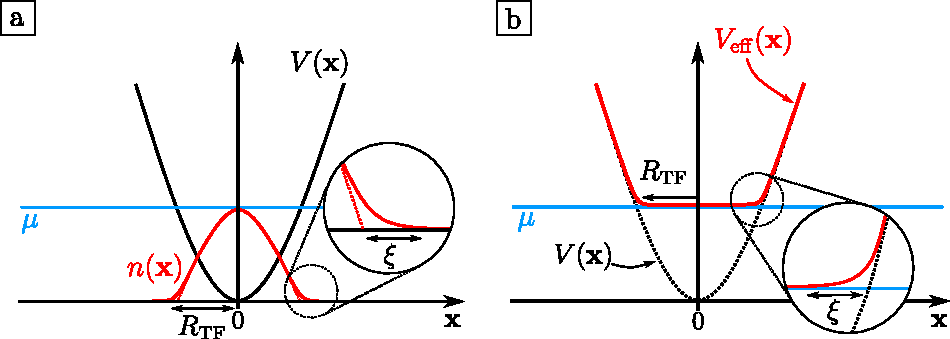
\includegraphics[width=\textwidth]{Fig/BEC_manip/thomas_fermi.pdf}
\caption{\textbf{a}: Profil de densité dans le régime de Thomas-Fermi. La densité est une parabole inversée, liée à la forme parabolique du potentiel. Sur les bords du condensat, la densité s'écarte de la parabole sur une longueur typique appelée longueur de cicatrisation. \textbf{b}: Potentiel effectif ressenti pour des particules individuelles. Ce potentiel effectif suit la forme du potentiel externe, et l'effet des interactions à l'intérieur du condensat écrante le potentiel externe par le potentiel chimique.}
\label{fig:thomas_fermi}
\end{figure}
Enfin, il est possible d'obtenir une expression pour le potentiel chimique \citep{pethick2008bose}: 
\begin{equation}
\mu=\frac{1}{2} \left( 15a N_{\mathbf{0}} \hb^2 \overline{\omega}^3 \right) ^{2/5} m^{1/5}
\end{equation}
et vaut environ $\mu/h\approx40$Hz pour notre expérience.

En réalité, l'approximation de Thomas-Fermi décrit bien les zones à l'intérieur des condensats, cependant, il existe une petite région sur les bords du condensat où la densité est faible, et donc l'énergie cinétique ne peut plus être négligée devant l'énergie d'interaction. Cette échelle de longueur s'appelle la longueur de cicatrisation, et est donnée par 
\begin{equation}
\xi=\sqrt{\frac{\hb^2}{n_{\mathbf{0}} mg}}
\end{equation}
avec $n_{\mathbf{0}}$ la ensité moyenne du condensat. $\xi$ représente donc la longueur sur laquelle le potentiel chimique n'écrante pas le potentiel externe.


\section{Processus d'interaction lumière-matière}
Précédemment, nous avons brièvement présenté le phénomène de condensation de Bose-Einstein ainsi que les principales propriétés d'un condensat. En particulier, nous avons identifié un critère de condensation, qui sert de ligne à atteindre sur notre dispositif. À présent, nous allons présenter les différents outils de manipulation d'atomes dont nous disposons pour obtenir la condensation d'un nuage de rubidium ${}^{87}$Rb.
\subsection{Le rubidium ${}^{87}$Rb}
Comme déjà mentionné plusieurs fois, l'espèce atomique utilisée sur notre expérimence est le rubidium ${}^{87}$Rb, le second isotope le plus abondant après le rubidium ${}^{85}$Rb (l'abondance naturelle du ${}^{87}$Rb est de 27.8\%). Il s'agit d'un alcalin (il possède donc un seul électron de valence) avec un spin nucléaire $I=3/2$. Le choix de cet isotope repose sur l'existence d'une transition optique cyclante dans sa raie $D$. De plus, sa longueur de diffusion $a_{\mathrm{s}}=5.3$nm résulte en des taux de collisions relativement élevés, permettant une thermalisation rapide du nuage. Il s'agit d'ailleurs de l'atome ayant été condensé en premier. \citep{anderson1995observation}

La raie $D$ est en réalité composée de deux transitions: la raie $D_1$ correspondant à la transition $4^2S_{1/2}\rightarrow5^2P_{1/2}$ à 895nm, et la raie $D_2$ correspondant à la transition $5^2S_{1/2}\rightarrow5^2P_{3/2}$ à 780nm. Sauf mention contraire, nous n'utiliserons que la raie $D_2$ dans la suite de ce manuscript, nos fréquences optiques se trouvant à 780nm. La structure hyperfine de l'état fondamental $5^2S_{1/2}$ consiste en deux niveaux hyperfins dégénérés $\left| F=1 \right\rangle$ et $\left| F=2 \right\rangle$ séparés de $\Delta_{\mathrm{hf}}=6.835$GHz. Chacun de ces états est composé de $2F+1$ sous-états Zeeman. 

\subsection{Potentiel dipolaire}
\begin{equation}
U_{\mathrm{dip}}(\mathbf{r})=\frac{3\pi c^2 \Gamma I(\mathbf{r})}{2 \omega_0^3} \left( \frac{1}{\omega - \omega_0} - \frac{1}{\omega + \omega_0} \right)
\end{equation}
\begin{equation}
\Gamma_{\mathrm{sp}}=\frac{3 \pi c^2 \omega^3 I(\mathbf{r})}{2\hb \omega_0^6} \left( \frac{\Gamma}{\omega-\omega_0}-\frac{\Gamma}{\omega+\omega_0} \right)^2
\end{equation}
\subsection{Force de pression de radiation}
\begin{equation}
s=\frac{I/I_{\mathrm{sat}}}{1+4(\omega-\omega_0)^2/\Gamma^2}
\end{equation}
\begin{equation}
I_{\mathrm{sat}}=\frac{\pi h c \Gamma}{3\lambda_o^3}
\end{equation}
\subsection{Potentiel magnétique}
\begin{equation}
\begin{array}{lll}
E_{F=2} &=\mu_{\mathrm{B}} g_{\mathrm{I}} m_F B + \frac{h \Delta_{\mathrm{hf}}}{2} \sqrt{1+ m_F \beta +\beta^2} \\
\\
E_{F=1} &=\mu_{\mathrm{B}} g_{\mathrm{I}} m_F B - \frac{h \Delta_{\mathrm{hf}}}{2} \sqrt{1+ m_F \beta +\beta^2}
\end{array}
\end{equation}
et $\beta=(g_{\mathrm{J}}-g_{\mathrm{I}})\mu_{\mathrm{B}} B/h \Delta_{\mathrm{hf}}$
\subsection{Couplage radio-fréquence} 

\section{Description d'un cycle expérimental}
\subsection{Première chambre}
\subsection{Chambre de science}
\subsection{Imagerie}

